\documentclass{fast-nuces-bs}

\usepackage{blindtext}
\usepackage{mathptmx}% Times Roman font
\usepackage[T1]{fontenc}
\usepackage{lipsum} 
\usepackage{sectsty}
\usepackage{tikz-uml}
\usepackage{titlesec}

% Information about the Thesis 
% -----------------------------------------------------------------------------
% (All are compulsory, do not delete any line other than author Information)
% For e.g., usually there are 3 students in a group, so leave authorone, 
% authortwo, and authorthree, and delete authorfour.
%%%%%%%%%%%%%%%%%%%%%%%%%%%%%%%%%%%%%%%%%%%%%%%%%%%%%%%%%%%%%%%%%%%%%%%%%%%%%%%
\department{Department of Computer Science}
\faculty{Artificial Intelligence}
\degreeyear{2023}
\degreemonth{November}
\degreename{Artificial Intelligence}
\campuscity{Karachi}
\authorone{Arooba Minhas}{21K-3094}
\authortwo{Bushra Khan}{21K-3081}
\authorthree{Alaina Usmani}{21K-3155}
\supervisor{Mr Faisal Ali}
\sessionduration{2023-2024}
\title{CONVEX HULL AND LINE SEGMENT ALGORITHMS IMPLEMENTATION AND ANALYSIS:}
%%%%%%%%%%%%%%%%%%%%%%%%%%%%%%%%%%%%%%%%%%%%%%%%%%%%%%%%%%%%%%%%%%%%%%%%%%%%%%%

%%%%%%%%%%%%%%%%%%%%%%%%%%%%%%%%%%%%%%%%%%%%%%%%%%%%%%%%%%%%%%%%%%%%%%%%%%%%%%
% Former document starts below this
\begin{document}
\begin{abstract}
This report presents the implementation and analysis of five convex hull algorithms—Brute Force, Jarvis March, Gramham Scan, Quick Elimination, and Andrew’s Algorithm, as well as a Line Segment Intersection algorithm using three different methods—Algebraic, CCW Computation, and Vector Cross Product. The implementation is carried out in Python, featuring a graphical user interface (GUI) for visualizing the results of both sets of algorithms. These algorithms are applied to respective sets of points and line segments, and their time and space complexities are thoroughly analyzed. The report aims to provide a comprehensive understanding of the performance characteristics and suitability of each algorithm in their respective problem domains.
\end{abstract}

\section{\textbf{Introduction}}

In the realm of computational geometry, convex hull algorithms stand as pivotal solutions to the challenge of identifying the convex hull within a given set of points. This report delves into the exploration of five distinct algorithms, each bringing its own unique approach to resolving the convex hull problem. Concurrently, the report also delves into the intricacies of Line Segment Intersection—a fundamental problem in computational geometry. This particular challenge involves determining the intersection of two provided line segments. Within this context, the report scrutinizes
three different algorithms, each offering its distinct methodology for tackling the Line Segment Intersection problem.

\section{\textbf{Programming Design}}
\subsection{}
\textbf{Convex Hull Algorithms:}

\textbf{0.2.1 Brute Force Convex Hull Algorithm:}

The Brute Force algorithm iteratively checks every triplet of points for a valid convex hull. This algorithm has a time
complexity of O(nˆ4) and a space complexity of O(n).
\textbf{0.2.2 Jarvis March Convex Hull Algorithm:}

Jarvis March, also known as the Gift Wrapping algorithm, selects the point with the lowest y-coordinate as the starting
point and iteratively selects the next point with the smallest polar angle. The time complexity of Jarvis March is
O(nˆ2), with a space complexity of O(n).
\textbf{0.2.3 Graham Scan Convex Hull Algorithm:}

The Graham Scan algorithm involves sorting points based on their polar angles and constructing the convex hull in a
counterclockwise manner. The time complexity of Graham Scan is O (n log n), and its space complexity is O(n).

\textbf{0.2.4 Quick Elimination Convex Hull Algorithm:}

Quick Elimination is an optimization of Graham Scan, where the point set is divided into smaller subsets, and Graham
Scan is applied to each subset. The time complexity is O (n log h), and the space complexity is O(n).

\textbf{0.2.5 Andrew’s Monotone Chain Convex Hull Algorithm:}

Andrew’s Algorithm sorts the points and computes the convex hull in two separate chains—lower and upper. The time
complexity is O (n log n), and the space complexity is O(n).


\section{\textbf{Line Segment Algorithms:}}

\subsection{}

\textbf{0.2.6 Algebraic Line Segment Intersection Algorithm:}

The Algebraic method calculates the slopes of the line segments and checks for intersection using algebraic equations.
The time complexity is dependent on the solution of a system of equations and is analyzed further in the results section.

\textbf{0.2.7 CCW Computation Line Segment Intersection Algorithm:}

The CCW (Counter Clockwise) computation method involves determining the orientation of three points. The algorithm checks the orientations of relevant point triplets to identify intersections efficiently.

\textbf{0.2.8 Vector Cross Product Line Segment Intersection Algorithm:}

The Vector Cross Product method utilizes vector operations to determine whether two line segments intersect. This
approach offers an alternative computational perspective.
\section{\textbf{Experimental Setup}}

Implemented in Python, the algorithms feature a graphical user interface (GUI) tailored for interactive visualization.
This GUI facilitates user engagement by enabling the input of points or line segments, the selection of a specific
algorithm, and the observation of the corresponding convex hull construction or intersection detection, depending on
the context.


\textbf{Experimental Setup Flow:}
\subsection{}
\textbf{Initialization:}

Set up the Python environment.
Import necessary libraries: tkinter for GUI, matplotlib for plotting, compare to key for sorting, time for measuring execution time, sys for memory usage, and sympy for algebraic computations. Graphical User Interface (GUI) Initialization:

\textbf{For Convex Hull Algorithms:}

Create a GUI for visualizing convex hull construction. Define a canvas for plotting points and convex hulls. Add buttons for each convex hull algorithm (Graham Scan, Jarvis March, Quick Elimination, Andrew's Algorithm, Brute Force). Include buttons for clearing points and displaying time and space complexities.
Design labels for time and space complexities.

\textbf{For Line Segment Intersection Algorithm:} 

Create a GUI for visualizing line segment intersections.
Define a canvas for plotting line segments and intersection points. Add buttons for different line segment intersection methods(Algebraic, CCW Computation, Vector Cross Product).Include buttons for adding points, clearing canvas, and displaying intersection results. Design labels for displaying intersection results.

\subsection{}
\textbf{Algorithm Implementation:}

Implement Convex Hull Algorithms in separate functions/classes.
Graham Scan, Jarvis March, Quick Elimination, Andrew's Algorithm, Brute Force. Implement Line Segment Intersection Algorithm in a separate class. Methods for Algebraic, CCW Computation, Vector Cross Product.

\subsection{}
\textbf{Experimental Execution:}

\textbf{For Convex Hull Algorithms:}

Measure the execution time using the time library.
Measure space complexity using sys.getsizeof().
Update the GUI labels with time and space complexity results.

\textbf{For Line Segment Intersection Algorithm:}

Implement methods to check intersection using different techniques.
Update the GUI labels with intersection results.

\section{\textbf{Results and Discussions:}}

\begin{figure}
    \centering
    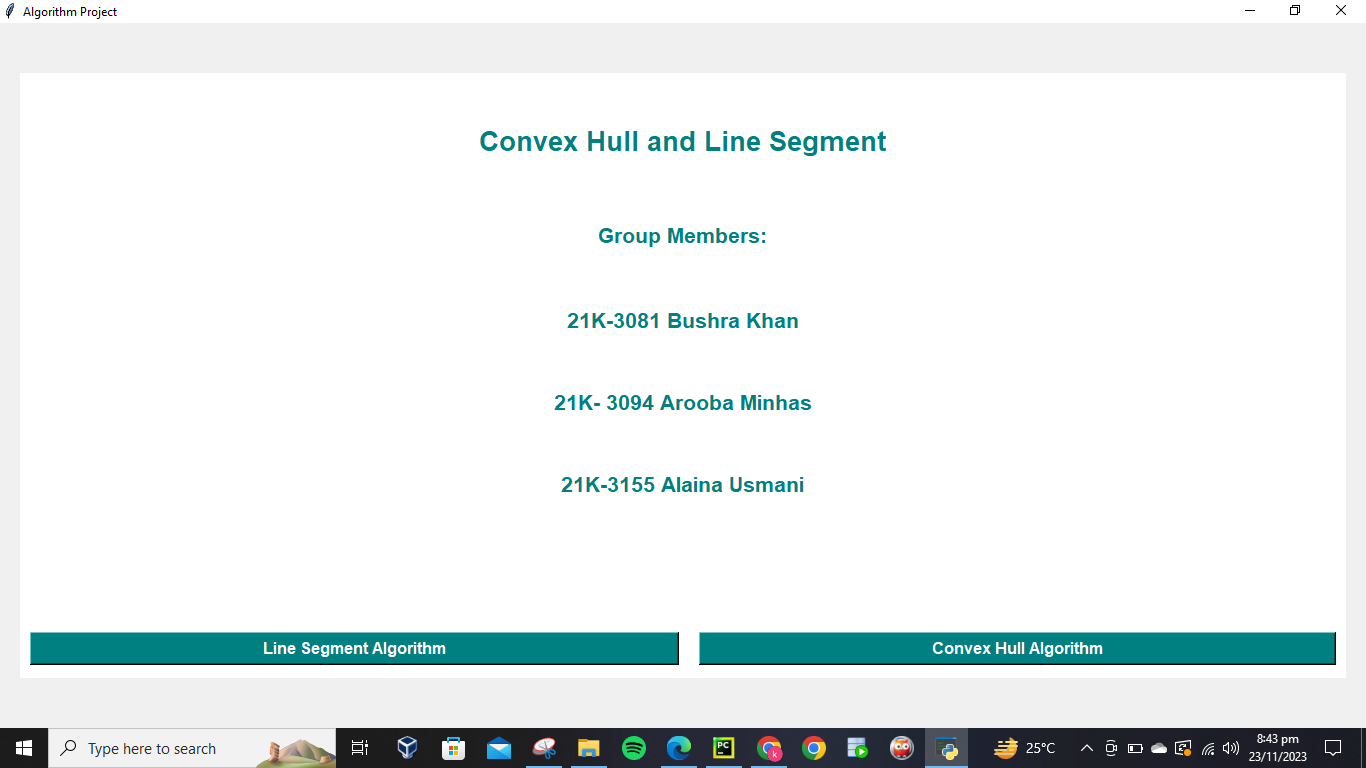
\includegraphics[width=1\linewidth]{p1.PNG}
    \caption{Title Page}
    \label{fig:enter-label}
\end{figure}

\begin{figure}
    \centering
    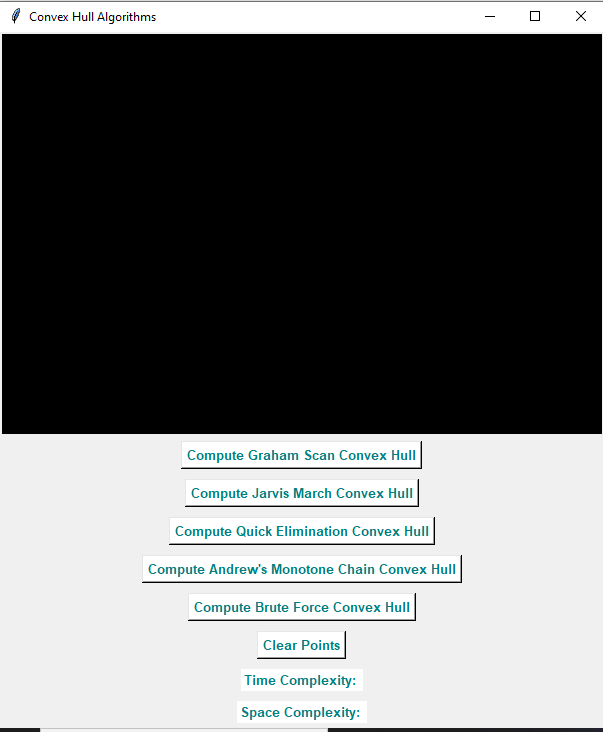
\includegraphics[width=1\linewidth]{p2.PNG}
    \caption{Convex Hull Algorithm Page}
    \label{fig:enter-label}
\end{figure}

\begin{figure}
    \centering
    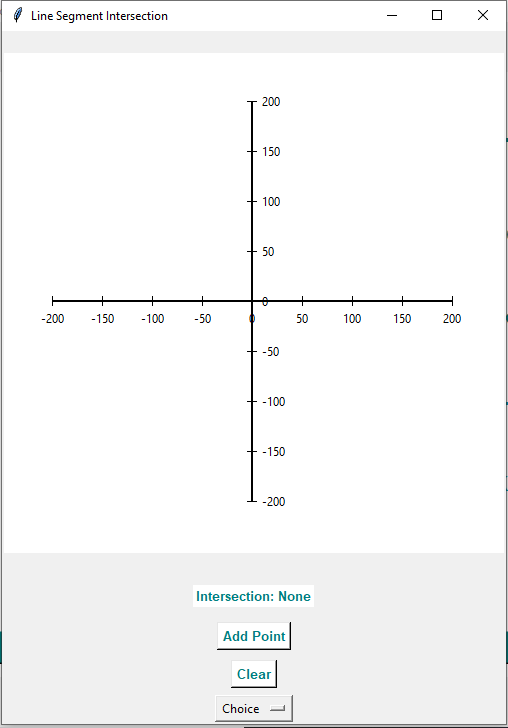
\includegraphics[width=1\linewidth]{p3.PNG}
    \caption{Line Segment Algorithm Page}
    \label{fig:enter-label}
\end{figure}


\section{Convex Hull Algorithms}

\subsection{\textbf{Brute Force Convex Hull:}}

The Brute Force algorithm exhibits high time complexity, making it impractical for large datasets. The resulting convex hull may be accurate, but the computational cost is significant.

\begin{figure}[h]
    \centering
    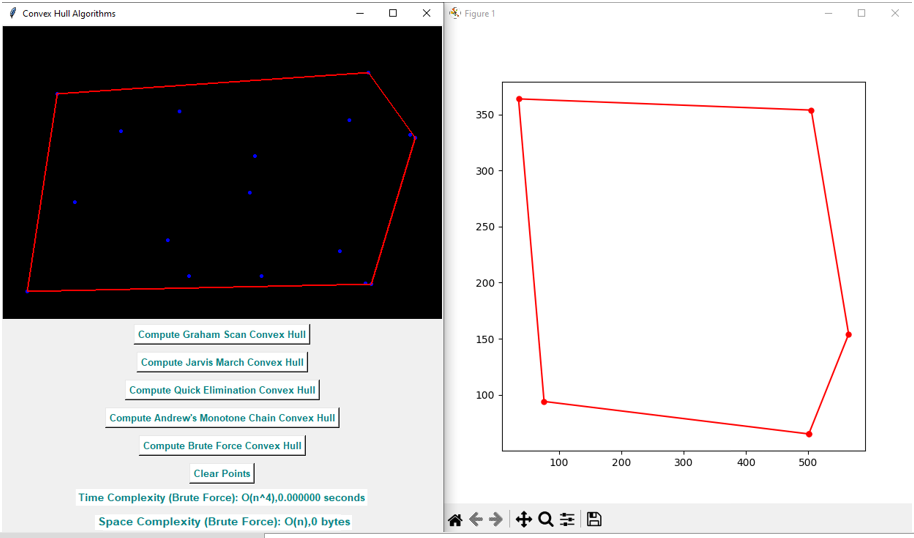
\includegraphics[width=1\linewidth]{bruteforce imsge.PNG}
    \caption{Brute Force}
    \label{fig:bruteforce}
\end{figure}

\vspace{10pt} 

\subsection{\textbf{Jarvis March Convex Hull:}}

Jarvis March provides a simple and intuitive solution with moderate time complexity. However, it may struggle with degenerate cases.

\begin{figure}[h]
    \centering
    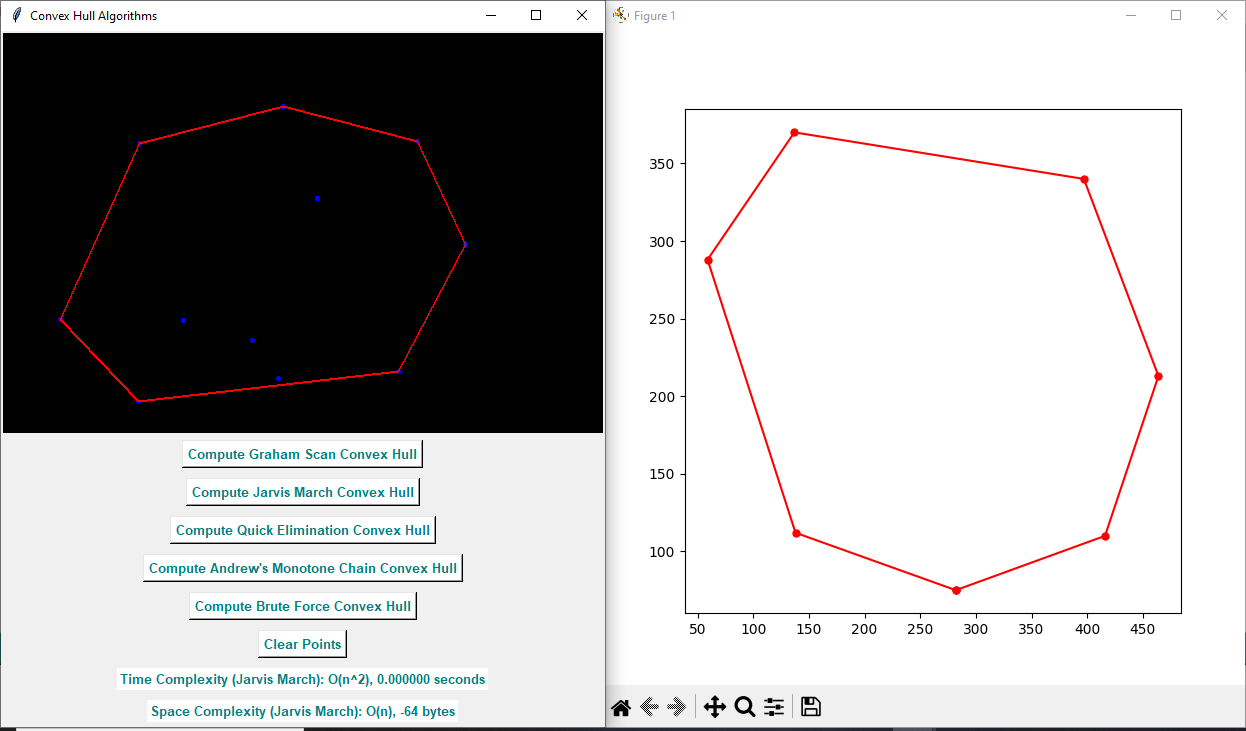
\includegraphics[width=1\linewidth]{jarvis.PNG}
    \caption{Jarvis March}
    \label{fig:jarvis}
\end{figure}

\vspace{10pt}

\subsection{\textbf{Graham Scan Convex Hull:}}

Graham Scan demonstrates improved efficiency, especially for large datasets. Its sorting step contributes to better overall performance.

\begin{figure}[h]
    \centering
    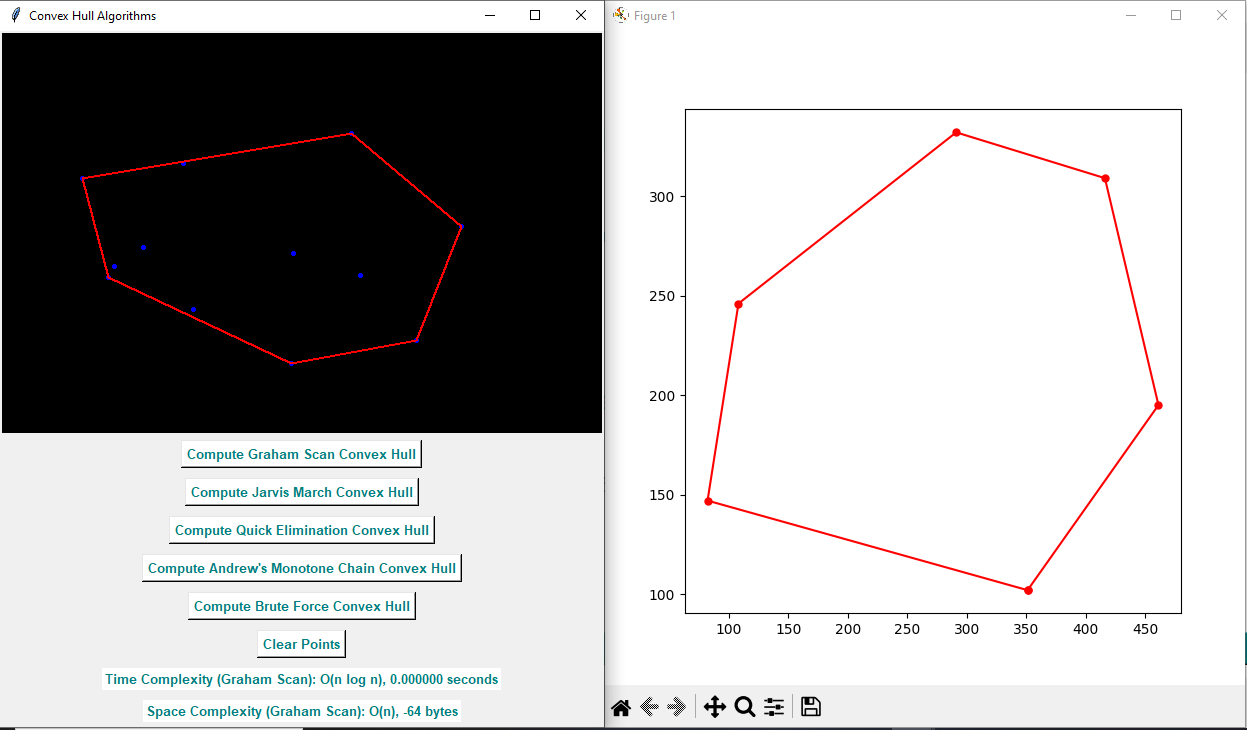
\includegraphics[width=1\linewidth]{grahamscan.PNG}
    \caption{Graham Scan}
    \label{fig:grahamscan}
\end{figure}

\vspace{10pt}




\subsection{\textbf{Quick Elimination Convex Hull:}}

Quick Elimination optimizes Graham Scan by dividing the point set into smaller subsets. This approach reduces the time complexity for specific cases.

\begin{figure}[h]
    \centering
    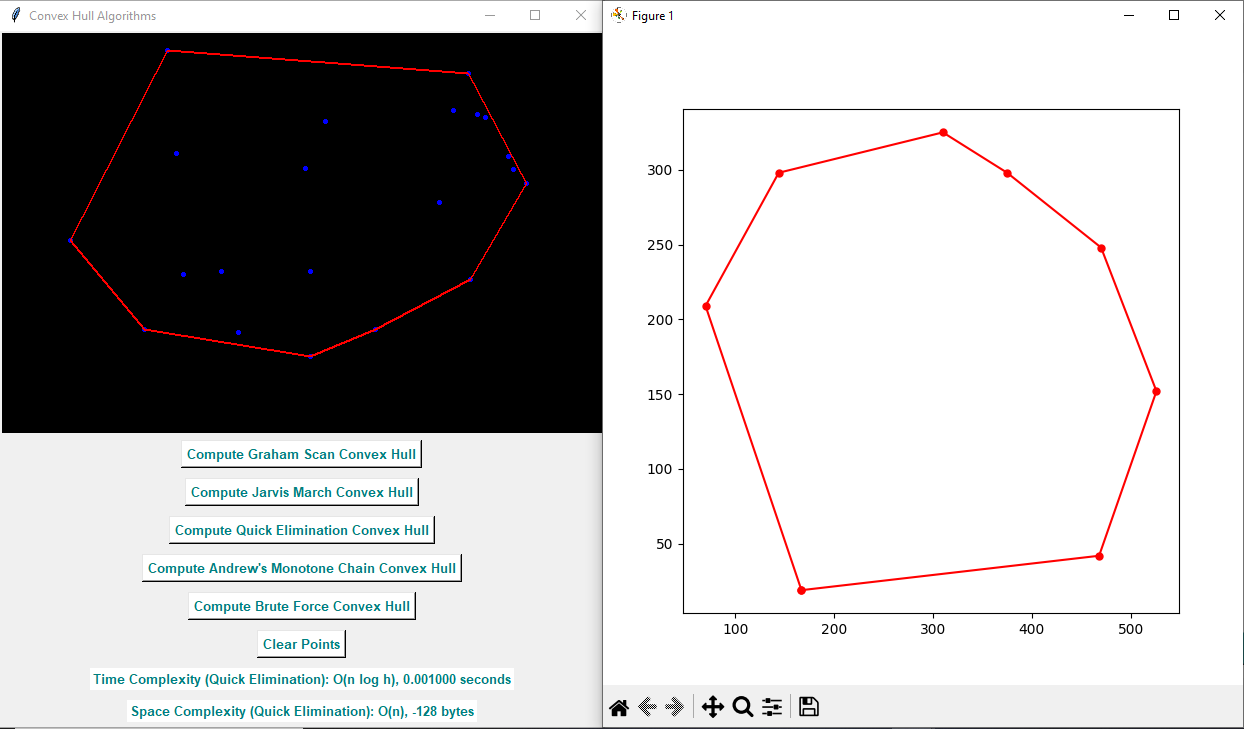
\includegraphics[width=1\linewidth]{quick elimination.PNG}
    \caption{Quick Elimination}
    \label{fig:quick elimination}
\end{figure}

\vspace{10pt}

\subsection{\textbf{Andrew’s Monotone Chain Convex Hull:}}

Andrew’s Algorithm offers a balance between efficiency and simplicity. It performs well for moderate-sized datasets.

\begin{figure}[h]
    \centering
    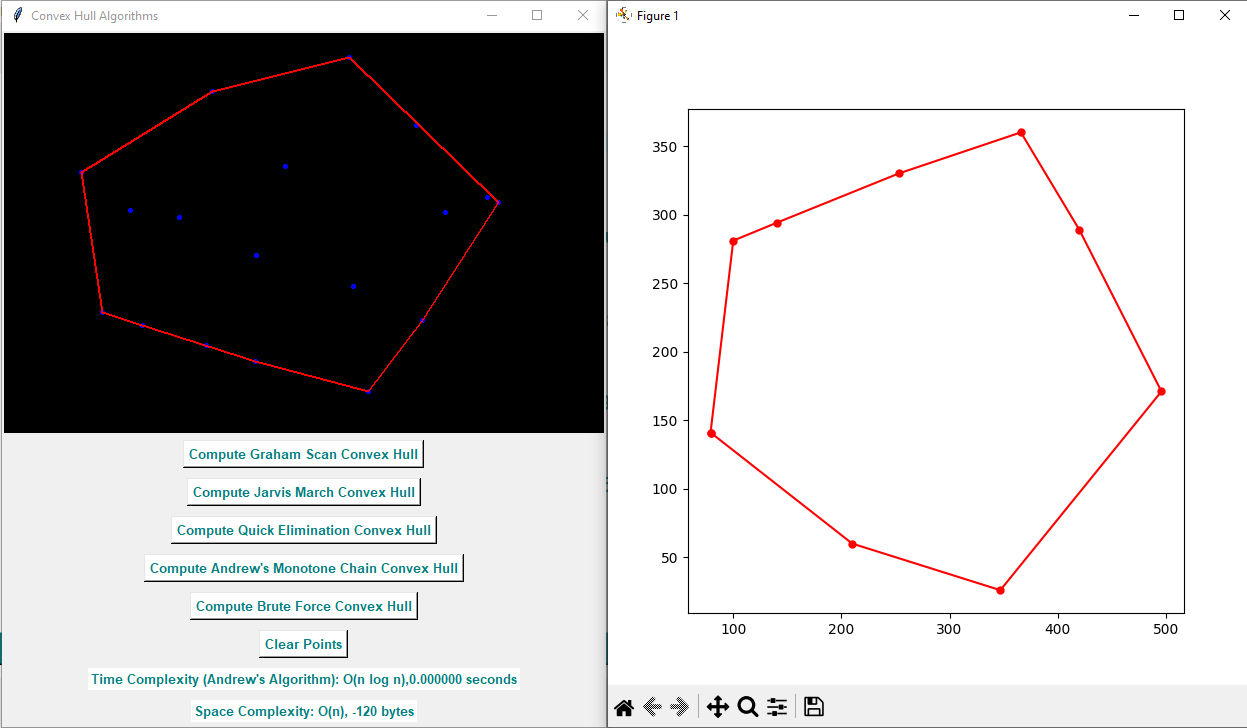
\includegraphics[width=1\linewidth]{andrew.PNG}
    \caption{Andrew's Monotone Chain}
    \label{fig:andrew}
\end{figure}


\section{Line Segment Algorithms}

\subsection{\textbf{Algebraic Line Segment Intersection:}}

The algebraic method exhibits a time complexity dependent on the solution of a system of equations. The accuracy of the intersection detection is high, but the computational cost may vary.

\begin{figure}[h]
    \centering
    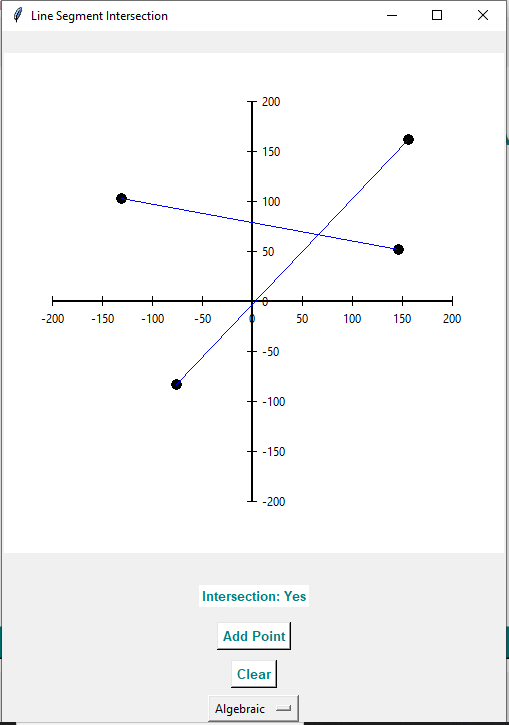
\includegraphics[width=1\linewidth]{algebraic.PNG}
    \caption{Algebraic}
    \label{fig:algebraic}
\end{figure}

\subsection{\textbf{CCW Computation Line Segment Intersection:}}

The CCW computation method provides efficient intersection detection by analyzing the orientations of point triplets. It proves to be a reliable algorithm for line segment intersection.

\begin{figure}[h]
    \centering
    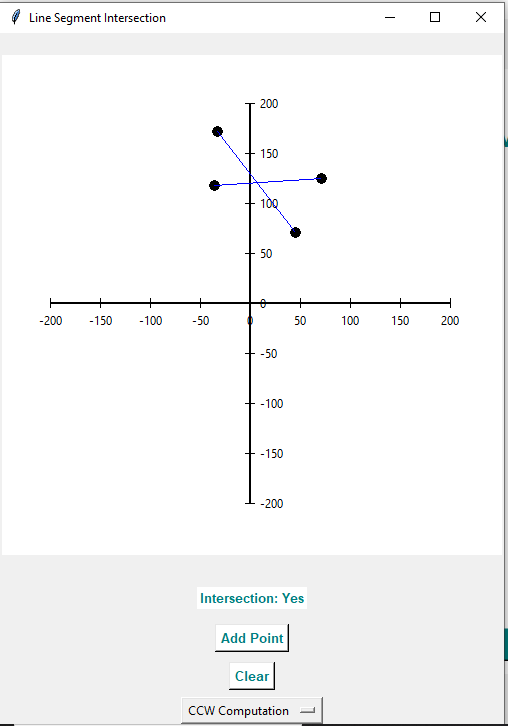
\includegraphics[width=1\linewidth]{ccw.PNG}
    \caption{CCW}
    \label{fig:ccw}
\end{figure}

\subsection{\textbf{Vector Cross Product Line Segment Intersection:}}

The Vector Cross Product method offers an alternative approach with efficient intersection detection. The algorithm’s performance is comparable to the CCW computation method.

\begin{figure}[h]
    \centering
    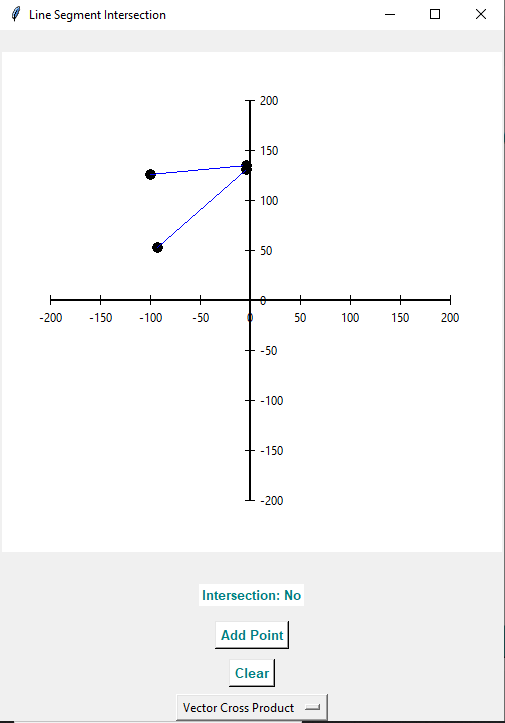
\includegraphics[width=1\linewidth]{vcp.PNG}
    \caption{Vector Cross Product}
    \label{fig:vcp}
\end{figure}

\section{\textbf{CONCLUSION:}}
In conclusion, the choice of a convex hull algorithm 
depends on the specific requirements of the 
application. For large datasets, Graham Scan and 
Quick Elimination prove to be efficient, while Jarvis 
March and Andrew's Algorithm strike a balance 
between performance and simplicity. Additionally, 
the choice of a Line Segment Intersection algorithm 
depends on specific requirements and considerations. 
The CCW computation and Vector Cross Product 
methods demonstrate efficient and reliable 
intersection detection. The algebraic method, while 
accurate, may have variable computational costs. The 
provided GUI enhances user interaction and 
visualization of the algorithms.

\section{\textbf{REFERENCES:}}

\begin{itemize}
    \item https://brilliant.org/wiki/convex-hull/
    \item https://www.youtube.com/watch?v=jjc92zWs1UA&t=316s&pp=ygUaY29udmV4IGh1bGwgdGhyb3VnaCBhbmRyZXc%3D
    \item https://www.youtube.com/watch v=B2AJoQSZf4M&pp=ygUaY29udmV4IGh1bGwgdGhyb3VnaCBhbmRyZXc%3D
\end{itemize}
\end{document}
